\subsubsection{Fonctionnement}
L'exponentiation modulaire est un moyen très efficace d'améliorer la vitesse de calcul d'un exposant.\\

Son fonctionnement est simple: on souhaite calculer un nombre \textit{a} à la puissance \textit{e} modulo un nombre \textit{m}. On commence par tester si \textit{e} modulo 2 est égal à 1. Si c'est le cas, on divise \textit{e} par 2, sinon on divise $e-1$ par 2. On continue ainsi jusqu'à ce que \textit{e} soit égal à 0.
Ainsi, à chaque itération l'exposant est divisé par 2.\\

Notre implémentation utilise les opérateurs binaires de Python. Dans notre fonction d'exponentiation modulaire, on utilise le code \textit{$e\&1$} pour tester si \textit{e} modulo 2 vaut 1. Pour diviser par 2, on effectue un décalage d'un bit à droite avec l'opérateur $\gg$.
Le nombre \textit{a} passé en argument est un nombre quelconque compris entre 1 et un nombre $p-1$ où \textit{p} est le nombre dont on souhaite déterminer la primalité. \textit{e} devient donc $p-1$ et \textit{m} devient \textit{p}. A chaque itération de boucle (sur l'exposant $p-1$), on donne à \textit{a} la valeur $a^2 $ modulo p.
\subsubsection{Benchmark}

Les captures suivantes montrent le temps de calcul du test de primalité utilisant l'exponentiation modulaire pour les mêmes nombres que ceux utilisés pour les benchmark du petit théorème de Fermat, à savoir: 733, 109 547, 3 000 000 et 9 999 991.\\

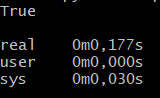
\includegraphics[scale=1]{images/expo1.png}
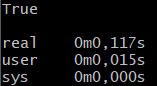
\includegraphics[scale=1]{images/expo2.png}
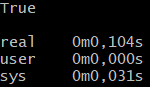
\includegraphics[scale=1]{images/expo3.png}
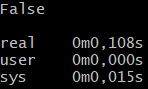
\includegraphics[scale=1]{images/expo4.png}
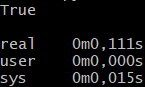
\includegraphics[scale=1]{images/expo5.png}

Cette fois-ci, contrairement au petit théorème de Fermat, le temps de calcul n'augmente pas. On peut donc déterminer si un nombre est premier très rapidement.\\
Ainsi le temps de calcul du test de primalité d'un très grand nombre comme 837 561 084 est de :

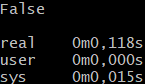
\includegraphics[scale=1]{images/expo6.png}

\subsubsection{Utilisation dans le petit théorème de Fermat}
Afin de rendre le calcul de primalité du petit théorème de Fermat plus performant, on peut remplacer le test $a^{p-1} \equiv 1$ (mod p) par un appel à la fonction d'exponentiation modulaire. L'exponentiation modulaire retourne combien de fois on a divisé l'exposant moins un par 2. Si un nombre est premier, on a effectué une et une seule division. Donc si la fonction retourne un nombre supérieur à 1, le nombre n'est pas premier.\\
Ainsi, comme on peut le voir en comparant les benchmarks, l'exponentiation modulaire permet de définir si un nombre est premier en un temps très petit et quel que soit ce nombre.